%%%%%%%%%%%%%%%%%%%%%%%%%%%%%%%%%%%%%%%%%
% Masters/Doctoral Thesis 
% LaTeX Template
% Version 2.5 (27/8/17)
%
% This template was downloaded from:
% http://www.LaTeXTemplates.com
%
% Version 2.x major modifications by:
% Vel (vel@latextemplates.com)
%
% This template is based on a template by:
% Steve Gunn (http://users.ecs.soton.ac.uk/srg/softwaretools/document/templates/)
% Sunil Patel (http://www.sunilpatel.co.uk/thesis-template/)
%
% Template license:
% CC BY-NC-SA 3.0 (http://creativecommons.org/licenses/by-nc-sa/3.0/)
%
%%%%%%%%%%%%%%%%%%%%%%%%%%%%%%%%%%%%%%%%%

%----------------------------------------------------------------------------------------
%	PACKAGES AND OTHER DOCUMENT CONFIGURATIONS
%----------------------------------------------------------------------------------------

\documentclass[
11pt, % The default document font size, options: 10pt, 11pt, 12pt
%oneside, % Two side (alternating margins) for binding by default, uncomment to switch to one side
english, % ngerman for German
singlespacing, % Single line spacing, alternatives: onehalfspacing or doublespacing
%draft, % Uncomment to enable draft mode (no pictures, no links, overfull hboxes indicated)
%nolistspacing, % If the document is onehalfspacing or doublespacing, uncomment this to set spacing in lists to single
%liststotoc, % Uncomment to add the list of figures/tables/etc to the table of contents
%toctotoc, % Uncomment to add the main table of contents to the table of contents
%parskip, % Uncomment to add space between paragraphs
%nohyperref, % Uncomment to not load the hyperref package
headsepline, % Uncomment to get a line under the header
%chapterinoneline, % Uncomment to place the chapter title next to the number on one line
%consistentlayout, % Uncomment to change the layout of the declaration, abstract and acknowledgements pages to match the default layout
]{MastersDoctoralThesis} % The class file specifying the document structure

\usepackage[utf8]{inputenc} % Required for inputting international characters
\usepackage[T1]{fontenc} % Output font encoding for international characters

\usepackage{mathpazo} % Use the Palatino font by default

\usepackage[backend=bibtex,style=authoryear,natbib=true]{biblatex} % Use the bibtex backend with the authoryear citation style (which resembles APA)

\addbibresource{bibliography.bib} % The filename of the bibliography

\usepackage[autostyle=true]{csquotes}
\usepackage{hyperref} % Required to generate language-dependent quotes in the bibliography

%----------------------------------------------------------------------------------------
%	MARGIN SETTINGS
%----------------------------------------------------------------------------------------

\geometry{
	paper=a4paper, % Change to letterpaper for US letter
	inner=2.5cm, % Inner margin
	outer=3.8cm, % Outer margin
	bindingoffset=.5cm, % Binding offset
	top=1.5cm, % Top margin
	bottom=1.5cm, % Bottom margin
	%showframe, % Uncomment to show how the type block is set on the page
}

%----------------------------------------------------------------------------------------
%	THESIS INFORMATION
%----------------------------------------------------------------------------------------

\thesistitle{Deep Learning For Predictive Maintenance} % Your thesis title, this is used in the title and abstract, print it elsewhere with \ttitle
\supervisor{Dr. Manuel \textsc{Sánchez-Montañés Isla}} % Your supervisor's name, this is used in the title page, print it elsewhere with \supname
\examiner{} % Your examiner's name, this is not currently used anywhere in the template, print it elsewhere with \examname
\degree{Software Engineer} % Your degree name, this is used in the title page and abstract, print it elsewhere with \degreename
\author{Hugo \textsc{Pérez Blasco}} % Your name, this is used in the title page and abstract, print it elsewhere with \authorname
\addresses{} % Your address, this is not currently used anywhere in the template, print it elsewhere with \addressname

\subject{Machine Learning} % Your subject area, this is not currently used anywhere in the template, print it elsewhere with \subjectname
\keywords{} % Keywords for your thesis, this is not currently used anywhere in the template, print it elsewhere with \keywordnames
\university{\href{http://mbitschool.academy/}{MBit School}} % Your university's name and URL, this is used in the title page and abstract, print it elsewhere with \univname
%\department{\href{http://department.university.com}{Department or School Name}} % Your department's name and URL, this is used in the title page and abstract, print it elsewhere with \deptname
%\group{\href{http://researchgroup.university.com}{Research Group Name}} % Your research group's name and URL, this is used in the title page, print it elsewhere with \groupname
%\faculty{\href{http://faculty.university.com}{Faculty Name}} % Your faculty's name and URL, this is used in the title page and abstract, print it elsewhere with \facname

\AtBeginDocument{
\hypersetup{pdftitle=\ttitle} % Set the PDF's title to your title
\hypersetup{pdfauthor=\authorname} % Set the PDF's author to your name
\hypersetup{pdfkeywords=\keywordnames} % Set the PDF's keywords to your keywords
}

\begin{document}

\frontmatter % Use roman page numbering style (i, ii, iii, iv...) for the pre-content pages

\pagestyle{plain} % Default to the plain heading style until the thesis style is called for the body content

%----------------------------------------------------------------------------------------
%	TITLE PAGE
%----------------------------------------------------------------------------------------

\begin{titlepage}
\begin{center}

\vspace*{.06\textheight}
{\scshape\LARGE \univname\par}\vspace{1.5cm} % University name
\textsc{\Large Advanced Deep Learning Master Dissertation}\\[0.5cm] % Thesis type

\HRule \\[0.4cm] % Horizontal line
{\huge \bfseries \ttitle\par}\vspace{0.4cm} % Thesis title
\HRule \\[1.5cm] % Horizontal line
 
\begin{minipage}[t]{0.4\textwidth}
\begin{flushleft} \large
\emph{Author:}\\
%\href{http://www.johnsmith.com}
{\authorname} % Author name - remove the \href bracket to remove the link
\end{flushleft}
\end{minipage}
\begin{minipage}[t]{0.4\textwidth}
\begin{flushright} \large
\emph{Supervisor:} \\
%\href{http://www.jamessmith.com}
{\supname} % Supervisor name - remove the \href bracket to remove the link
\end{flushright}
\end{minipage}\\[3cm]
 
\vfill

%\large \textit{A thesis submitted in fulfillment of the requirements\\ for the degree of \degreename}\\[0.3cm] % University requirement text
%\textit{in the}\\[0.4cm]
%\groupname\\\deptname\\[2cm] % Research group name and department name
 
\vfill

{\large \today}\\[4cm] % Date
%\includegraphics{Logo} % University/department logo - uncomment to place it
 
\vfill
\end{center}
\end{titlepage}

%----------------------------------------------------------------------------------------
%	DECLARATION PAGE
%----------------------------------------------------------------------------------------

%\begin{declaration}
%\addchaptertocentry{\authorshipname} % Add the declaration to the table of contents
%\noindent I, \authorname, declare that this thesis titled, \enquote{\ttitle} and the work presented in it are my own. I confirm that:
%
%\begin{itemize}
%\item This work was done wholly or mainly while in candidature for a research degree at this University.
%\item Where any part of this thesis has previously been submitted for a degree or any other qualification at this University or any other institution, this has been clearly stated.
%\item Where I have consulted the published work of others, this is always clearly attributed.
%\item Where I have quoted from the work of others, the source is always given. With the exception of such quotations, this thesis is entirely my own work.
%\item I have acknowledged all main sources of help.
%\item Where the thesis is based on work done by myself jointly with others, I have made clear exactly what was done by others and what I have contributed myself.\\
%\end{itemize}
%
%\noindent Signed:\\
%\rule[0.5em]{25em}{0.5pt} % This prints a line for the signature
%
%\noindent Date:\\
%\rule[0.5em]{25em}{0.5pt} % This prints a line to write the date
%\end{declaration}
%
%\cleardoublepage

%----------------------------------------------------------------------------------------
%	QUOTATION PAGE
%----------------------------------------------------------------------------------------

%\vspace*{0.2\textheight}
%
%\noindent\enquote{\itshape Thanks to my solid academic training, today I can write hundreds of words on virtually any topic without possessing a shred of information, which is how I got a good job in journalism.}\bigbreak
%
%\hfill Dave Barry

%----------------------------------------------------------------------------------------
%	ABSTRACT PAGE
%----------------------------------------------------------------------------------------

\begin{abstract}
\addchaptertocentry{\abstractname} % Add the abstract to the table of contents
Predictive maintenance encompasses a variety of topics, including but not limited to: failure prediction, failure diagnosis (root cause analysis), failure detection, failure type classification, and recommendation of mitigation or maintenance actions after failure \parencite{Reference1}.

Predictive Maintenance is also a domain where data is collected over time to monitor the state of an asset with the goal of finding patterns to predict failures which can also benefit from certain deep learning algorithms \parencite{Reference2}.
This study uses simulated aircraft sensor values to predict when an aircraft engine will fail in the future so that maintenance can be planned in advance \parencite{Reference3}.

The goal of this dissertation if to do a trade-off over the different deep learning architectures and models that compound the current state of the art concerning the prediction and classification over time series data.
\end{abstract}

%----------------------------------------------------------------------------------------
%	ACKNOWLEDGEMENTS
%----------------------------------------------------------------------------------------

%\begin{acknowledgements}
%\addchaptertocentry{\acknowledgementname} % Add the acknowledgements to the table of contents
%The acknowledgments and the people to thank go here, don't forget to include your project advisor\ldots
%\end{acknowledgements}

%----------------------------------------------------------------------------------------
%	LIST OF CONTENTS/FIGURES/TABLES PAGES
%----------------------------------------------------------------------------------------

\tableofcontents % Prints the main table of contents

\listoffigures % Prints the list of figures

\listoftables % Prints the list of tables

%----------------------------------------------------------------------------------------
%	ABBREVIATIONS
%----------------------------------------------------------------------------------------

\begin{abbreviations}{ll} % Include a list of abbreviations (a table of two columns)

\textbf{LAH} & \textbf{L}ist \textbf{A}bbreviations \textbf{H}ere\\
\textbf{WSF} & \textbf{W}hat (it) \textbf{S}tands \textbf{F}or\\

\end{abbreviations}

%----------------------------------------------------------------------------------------
%	PHYSICAL CONSTANTS/OTHER DEFINITIONS
%----------------------------------------------------------------------------------------

%\begin{constants}{lr@{${}={}$}l} % The list of physical constants is a three column table

% The \SI{}{} command is provided by the siunitx package, see its documentation for instructions on how to use it

%Speed of Light & $c_{0}$ & \SI{2.99792458e8}{\meter\per\second} (exact)\\
%Constant Name & $Symbol$ & $Constant Value$ with units\\

%\end{constants}

%----------------------------------------------------------------------------------------
%	SYMBOLS
%----------------------------------------------------------------------------------------

%\begin{symbols}{lll} % Include a list of Symbols (a three column table)

%$a$ & distance & \si{\meter} \\
%$P$ & power & \si{\watt} (\si{\joule\per\second}) \\
%Symbol & Name & Unit \\

%\addlinespace % Gap to separate the Roman symbols from the Greek

%$\omega$ & angular frequency & \si{\radian} \\

%\end{symbols}

%----------------------------------------------------------------------------------------
%	DEDICATION
%----------------------------------------------------------------------------------------

%\dedicatory{For/Dedicated to/To my\ldots}

%----------------------------------------------------------------------------------------
%	THESIS CONTENT - CHAPTERS
%----------------------------------------------------------------------------------------

\mainmatter % Begin numeric (1,2,3...) page numbering

\pagestyle{thesis} % Return the page headers back to the "thesis" style

% Include the chapters of the thesis as separate files from the Chapters folder
% Uncomment the lines as you write the chapters

% Chapter 1

\chapter{Objectives} % Main chapter title

\label{Chapter1} % For referencing the chapter elsewhere, use \ref{Chapter1} 

%----------------------------------------------------------------------------------------

% Define some commands to keep the formatting separated from the content 
\newcommand{\keyword}[1]{\textbf{#1}}
\newcommand{\tabhead}[1]{\textbf{#1}}
\newcommand{\code}[1]{\texttt{#1}}
\newcommand{\file}[1]{\texttt{\bfseries#1}}
\newcommand{\option}[1]{\texttt{\itshape#1}}

%----------------------------------------------------------------------------------------

\section{Problem Description}
Aircraft lifetime and maintenance is a recurrent problem for companies due to its high costs.
Being able to predict when an aircraft is going to have failures or malfunctioning is a key topic for improving costs and performance of this machines.

The scenario uses data from simulated aircraft sensor to predict when an aircraft engine will fail in the future.
Two different approaches are used for this problem:

\begin{itemize}
\item A regression models that manages to answer the question: How many more cycles an in-service engine will last before it fails?
\item A binary classification model that manages to answer the question: Is this engine going to fail within a specific number of time cycles?
\end{itemize}

%----------------------------------------------------------------------------------------

\section{Data Summary}\label{sec:data-summary}

The data provided is divided in three different sets:

\subsection{Training data}\label{subsec:training-data}

The training data consists of multiple multivariate time series with "cycle" as the time unit, together with 21 sensor readings for each cycle.
Each time series can be assumed as being generated from a different engine of the same type.
Each engine is assumed to start with different degrees of initial wear and manufacturing variation, and this information is unknown to the user.
In this simulated data, the engine is assumed to be operating normally at the start of each time series.
It starts to degrade at some point during the series of the operating cycles.
The degradation progresses and grows in magnitude.
When a predefined threshold is reached, then the engine is considered unsafe for further operation.
In other words, the last cycle in each time series can be considered as the failure point of the corresponding engine.
Taking the sample training data shown in the following table as an example, the engine with id=1 fails at cycle 192.

\begin{table}
\caption{Training Data}
\label{tab:training-data}
\centering
\begin{tabular}{l l l l l l l l l }
\toprule
\tabhead{Id} & \tabhead{Cycle} & \tabhead{Setting 1} & \tabhead{Setting 2} & \tabhead{S1} & \tabhead{S2} & \tabhead{S3} & \tabhead{...} \\
\midrule
1 & 1   & -0.0007  & -0.0004 & 100.0 & 518.67 & 641.82 & ... \\
1 & 2   & 0.0019   & -0.0003 & 100.0 & 518.67 & 642.15 & ... \\
1 & 3   & -0.0043  & 0.0003  & 100.0 & 518.67 & 642.35 & ... \\
... & ... & & & &  & & ... \\
1 & 191 & 0        & -0.0004 & 100.0 & 518.67 & 643.34 & ... \\
1 & 192 & 0.0009   & 0       & 100.0 & 518.67 & 643.54 & ... \\
2 & 1   & -0.0018  & 0.0006  & 100.0 & 518.67 & 641.89 & ... \\
2 & 2   & 0.0009   & -0.0003 & 100.0 & 518.67 & 641.82 & ... \\
2 & 3   & 0.0018   & 0.0003  & 100.0 & 518.67 & 641.55 & ... \\
... & ... & & & &  & & ... \\
\bottomrule\\
\end{tabular}
\end{table}

\subsection{Test data}\label{subsec:text-data}

The testing data has the same data schema as the training data.
The only difference is that the data does not indicate when the failure occurs (in other words, the last time period does NOT represent the failure point).
Taking the sample testing data shown in the following table as an example, the engine with id=1 runs from cycle 1 through cycle 31.
It is not shown how many more cycles this engine can last before it fails.

\begin{table}
\caption{Test Data}
\label{tab:test-data}
\centering
\begin{tabular}{l l l l l l l l l }
\toprule
\tabhead{Id} & \tabhead{Cycle} & \tabhead{Setting 1} & \tabhead{Setting 2} & \tabhead{S1} & \tabhead{S2} & \tabhead{S3} & \tabhead{...} \\
\midrule
1 & 1  & 0.0023   & 0.0003  & 100.0 & 518.67 & 643.02 & ... \\
1 & 2  & -0.0027  & -0.0003 & 100.0 & 518.67 & 641.71 & ... \\
1 & 3  & 0.0003   & 0.0001  & 100.0 & 518.67 & 642.46 & ... \\
... & ... & & & &  & & ... \\
1 & 30 & -0.0025  & 0.0004  & 100.0 & 518.67 & 642.79 & ... \\
1 & 31 & -0.0006  & 0.0004  & 100.0 & 518.67 & 642.58 & ... \\
2 & 1  & -0.0009  & 0.0006  & 100.0 & 518.67 & 641.89 & ... \\
2 & 2  & -0.0011  & 0.0002  & 100.0 & 518.67 & 642.51 & ... \\
2 & 3  & 0.0002   & 0.0003  & 100.0 & 518.67 & 642.58 & ... \\
... & ... & & & &  & & ... \\
\bottomrule\\
\end{tabular}
\end{table}

\subsection{Ground truth data}\label{subsec:ground-truth-data}
The ground truth data provides the number of remaining working cycles for the engines in the testing data.
Taking the sample ground truth data shown in the following table as an example, the engine with id=1 in the testing data can run another 112 cycles before it fails.

\begin{table}
\caption{Ground Truth Data}
\label{tab:ground-truth-data}
\centering
\begin{tabular}{l}
\toprule
\tabhead{RUL} \\
\midrule
112 \\
98 \\
69 \\
82 \\
91 \\
... \\
\bottomrule\\
\end{tabular}
\end{table}

%----------------------------------------------------------------------------------------

\section{Dissertation goals}

Once the data and the problem to solve is known, the goal of this dissertation is to expose and analyze the different approaches and alternatives used for the problem resolution.

All of the different methodologies, technical solutions and results will be explained step by step and compared within each other.

Finally some conclusions must be extracted in order to clarify which one is the best approach to solve the problem concerning this dissertation context.


%% Chapter Template

\chapter{Methodology and Techniques} % Main chapter title

\label{Chapter2}

%----------------------------------------------------------------------------------------
%	SECTION 1
%----------------------------------------------------------------------------------------

\section{Deep Learning for sequence processing}

This dissertation is focused on the use of Deep Learning techniques to solve predictive maintenance problems.

Some of this techniques are going to be used to solve the problem exposed in chapter \ref{Chapter1}.

This methodologies and techniques are chosen based on the state-of-art of the topic and also on its frequency of use.


%-----------------------------------
%	SUBSECTION 1
%-----------------------------------
\subsection{Study methodology}

The methodology for the study follows the next steps:

\begin{itemize}
    \item Data analysis and pre-processing.
    \item Technical solution and model definition.
    \item Model and data visualization.
    \item Analysis of the results.
    \item Hyper-parameters and model adjustment
    \item Conclusions
\end{itemize}

%-----------------------------------
%	SUBSECTION 2
%-----------------------------------

\subsection{Trade-off}

The results of each approach and technique will be compared in a trade-off extracting conclusion about its feasibility to solve the exposed problem.

Also, future directions and improvements will be discussed in agreement with the results of the dissertation.
%% Chapter Template

\chapter{Data Analysis and Pre-processing} % Main chapter title

\label{Chapter3}

%----------------------------------------------------------------------------------------
%	SECTION 1
%----------------------------------------------------------------------------------------

\section{Data labelling}

The first step is to generate the labels required to train the model.
Two different labels must be generated for each question we want to answer:

\begin{itemize}
    \item Remaining Useful Life (RUL) for the regression problem.
    \item Boolean flag indicating if the RUL is less than an specific cycle value.
\end{itemize}

%-----------------------------------
%	SUBSECTION 1
%-----------------------------------
\subsection{Remaining Useful Life}

In order to face the regression model to answer the question \textit{how many more cycles an in-service engine will last before it fails?} each entrance of the train dataset must include the number of remaining cycles until the aircraft fails.

This way, all the rows associated with the same aircraft identifier will have a decreasing number for this field. In the last step, where the cycle number represents the moment the aircraft fails, the RUL must be 0. See table \ref{tab:training-data-rul}

\begin{table}
\caption{Training Data with RUL column}
\label{tab:training-data-rul}
\centering
\begin{tabular}{l l l l l l l}
\toprule
\tabhead{Id} & \tabhead{Cycle} & \tabhead{Setting 1} & \tabhead{Setting 2} & \tabhead{S1} & \tabhead{...} & \tabhead{RUL}\\
\midrule
1 & 1   & -0.0007  & -0.0004 & 100.0 & ... & 191\\
1 & 2   & 0.0019   & -0.0003 & 100.0 & ... & 190\\
1 & 3   & -0.0043  & 0.0003  & 100.0 & ... & 189\\
... & ... & & & &  & ... \\
1 & 191 & 0        & -0.0004 & 100.0 & ... & 1\\
1 & 192 & 0.0009   & 0       & 100.0 & ... & 0\\
2 & 1   & -0.0018  & 0.0006  & 100.0 & ... & 286\\
2 & 2   & 0.0009   & -0.0003 & 100.0 & ... & 285\\
2 & 3   & 0.0018   & 0.0003  & 100.0 & ... & 284\\
... & ... & & & & & ... \\
\bottomrule\\
\end{tabular}
\end{table}

%-----------------------------------
%	SUBSECTION 2
%-----------------------------------

\subsection{Failure Cycle Window}

In the case of the binary classification model, the question to answer is \textit{is this engine going to fail within w1 cycles?}.

The w1 represents the window of cycles that we want to take in account to classify. In this dissertation the number of cycles will be set to 30.

Along with the RUL, it is possible to generate a label (label1) for each entrance indicating if the aircraft failed on this cycle window. To calculate it, just set to 1 ("true") all the RUL values lesser than w1. See table \ref{tab:training-data-w1}

\begin{table}
\caption{Training Data with label for classification}
\label{tab:training-data-w1}
\centering
\begin{tabular}{l l l l l l l l}
\toprule
\tabhead{Id} & \tabhead{Cycle} & \tabhead{Setting 1} & \tabhead{Setting 2} & \tabhead{S1} & \tabhead{...} & \tabhead{RUL} & \tabhead{label1}\\
\midrule
1 & 1   & -0.0007  & -0.0004 & 100.0 & ... & 191 & 0\\
1 & 2   & 0.0019   & -0.0003 & 100.0 & ... & 190 & 0\\
1 & 3   & -0.0043  & 0.0003  & 100.0 & ... & 189 & 0\\
... & ... & & & &  & & ... \\
1 & 191 & 0        & -0.0004 & 100.0 & ... & 1 & 1\\
1 & 192 & 0.0009   & 0       & 100.0 & ... & 0 & 1\\
2 & 1   & -0.0018  & 0.0006  & 100.0 & ... & 286 & 0\\
2 & 2   & 0.0009   & -0.0003 & 100.0 & ... & 285 & 0\\
2 & 3   & 0.0018   & 0.0003  & 100.0 & ... & 284 & 0\\
... & ... & & & & & & ... \\
\bottomrule\\
\end{tabular}
\end{table}

%----------------------------------------------------------------------------------------
%	SECTION 2
%----------------------------------------------------------------------------------------

\section{Feature Engineering and Normalization}

The information of the aircraft for each time step is formed by 21 different sensor and 3 setting numerical values.
The distribution of this values is shown in the figure \ref{fig:data-distribution}.

The data distribution shows that most of the sensor data follows a gaussian distribution, avoiding the existence of outliers. With this premise and also taking in account that some of the value ranges can take negative values, the normalization method chosen is min max scaler.

Min max scaler normalization transforms the values in the distribution to the range [0-1]. This normalization is required to avoid the network to priorize on features with higher values and also to avoid exploding gradient problems.

\begin{figure}
    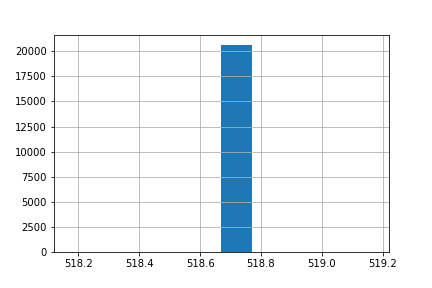
\includegraphics[width=.24\textwidth]{Figures/s1}\hfill
    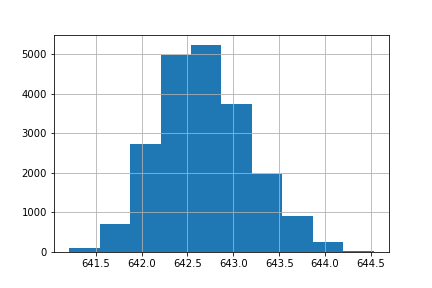
\includegraphics[width=.24\textwidth]{Figures/s2}\hfill
    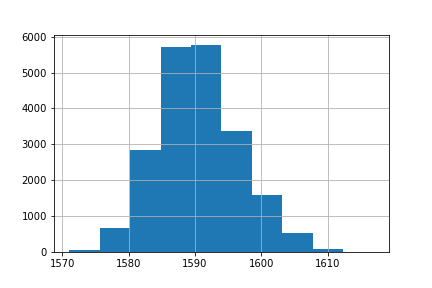
\includegraphics[width=.24\textwidth]{Figures/s3}\hfill
    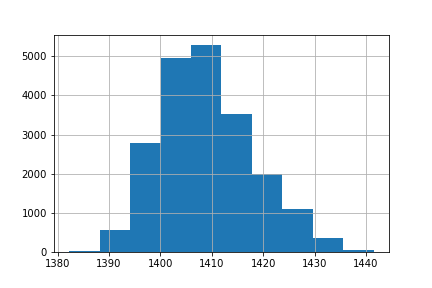
\includegraphics[width=.24\textwidth]{Figures/s4}
    \\[\smallskipamount]
    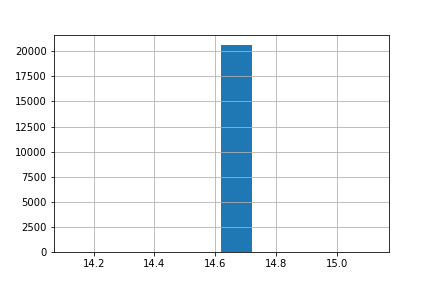
\includegraphics[width=.24\textwidth]{Figures/s5}\hfill
    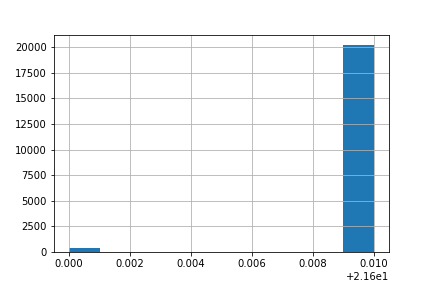
\includegraphics[width=.24\textwidth]{Figures/s6}\hfill
    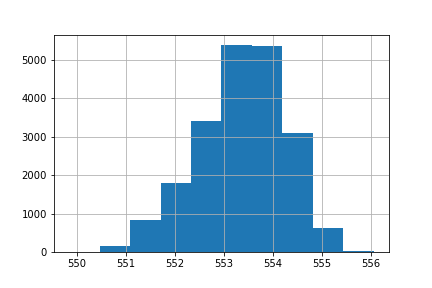
\includegraphics[width=.24\textwidth]{Figures/s7}\hfill
    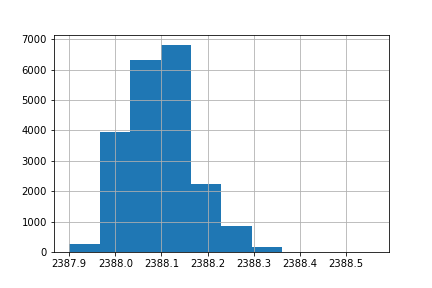
\includegraphics[width=.24\textwidth]{Figures/s8}
    \\[\smallskipamount]
    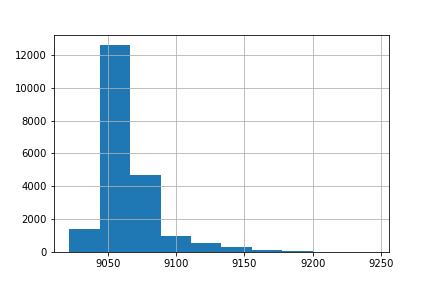
\includegraphics[width=.24\textwidth]{Figures/s9}\hfill
    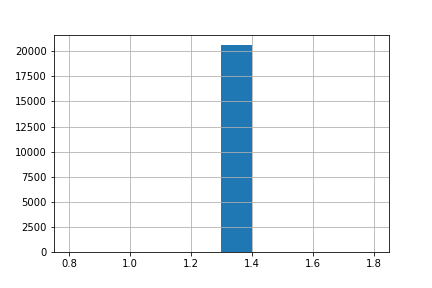
\includegraphics[width=.24\textwidth]{Figures/s10}\hfill
    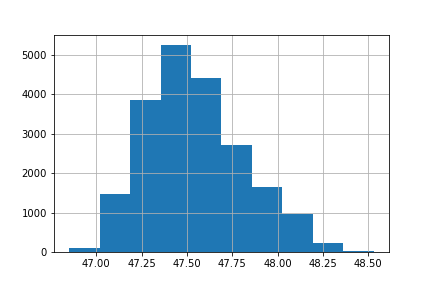
\includegraphics[width=.24\textwidth]{Figures/s11}\hfill
    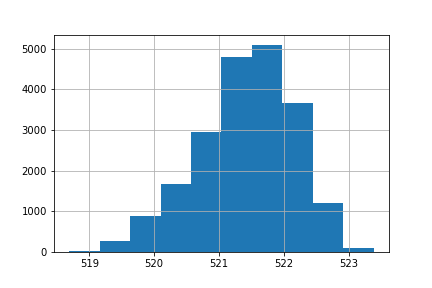
\includegraphics[width=.24\textwidth]{Figures/s12}
    \\[\smallskipamount]
    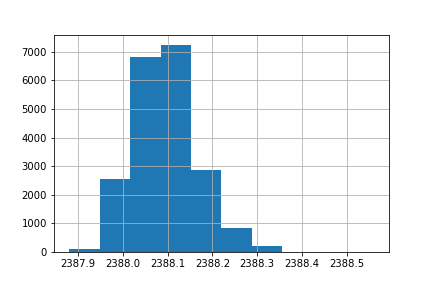
\includegraphics[width=.24\textwidth]{Figures/s13}\hfill
    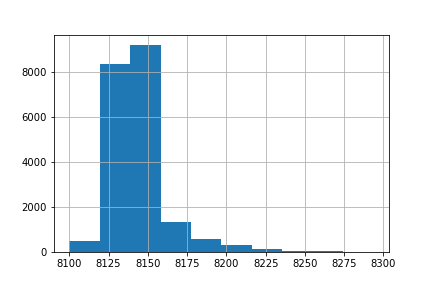
\includegraphics[width=.24\textwidth]{Figures/s14}\hfill
    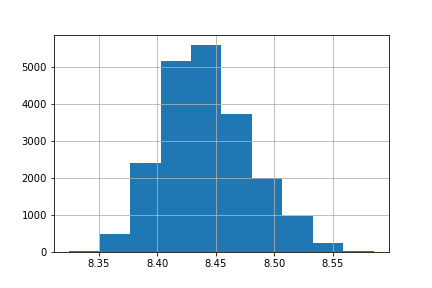
\includegraphics[width=.24\textwidth]{Figures/s15}\hfill
    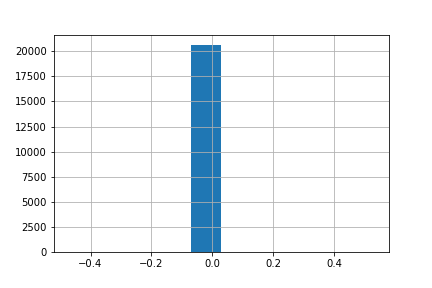
\includegraphics[width=.24\textwidth]{Figures/s16}
    \\[\smallskipamount]
    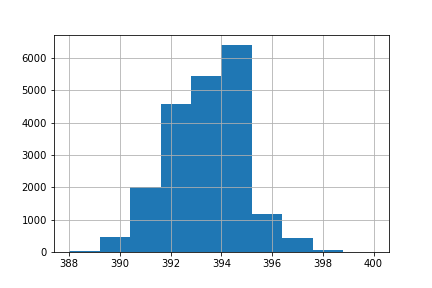
\includegraphics[width=.24\textwidth]{Figures/s17}\hfill
    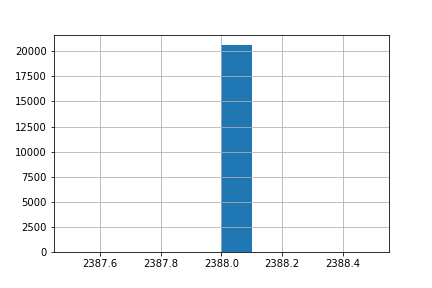
\includegraphics[width=.24\textwidth]{Figures/s18}\hfill
    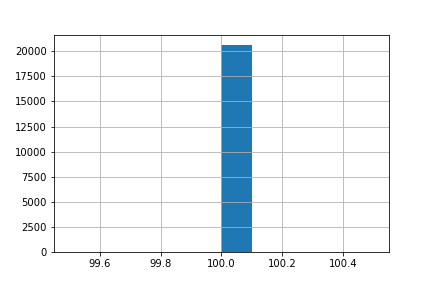
\includegraphics[width=.24\textwidth]{Figures/s19}\hfill
    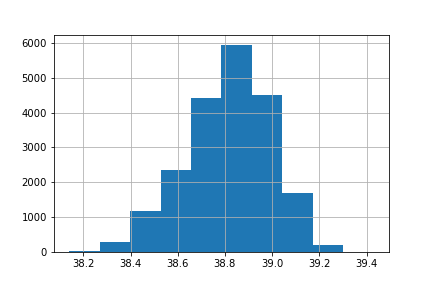
\includegraphics[width=.24\textwidth]{Figures/s20}
    \\[\smallskipamount]
    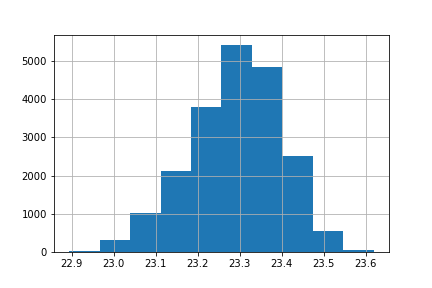
\includegraphics[width=.24\textwidth]{Figures/s21}\hfill
    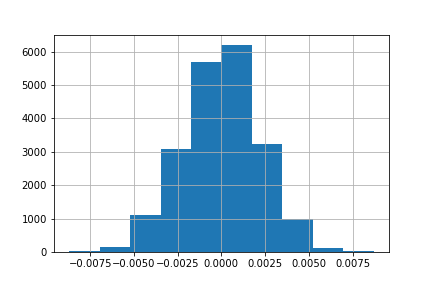
\includegraphics[width=.24\textwidth]{Figures/setting1}\hfill
    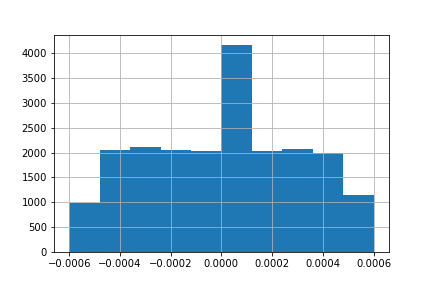
\includegraphics[width=.24\textwidth]{Figures/setting2}\hfill
    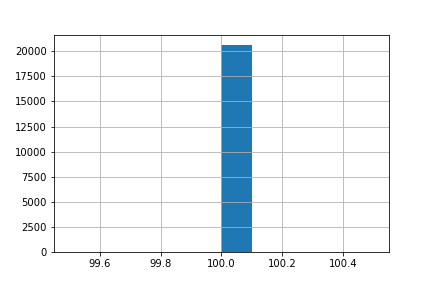
\includegraphics[width=.24\textwidth]{Figures/setting3}
    \caption{Sensor data distribution}\label{fig:data-distribution}
\end{figure}

%% Chapter Template

\chapter{Long Short-Term Memory} % Main chapter title

\label{Chapter4} % Change X to a consecutive number; for referencing this chapter elsewhere, use \ref{ChapterX}

%----------------------------------------------------------------------------------------
%	SECTION 1
%----------------------------------------------------------------------------------------

\section{Understanding LSTMs}

Long Short Term Memory networks – usually just called \textit{LSTMs} – are a special kind of RNN, capable of learning long-term dependencies. They were introduced by Hochreiter and Schmidhuber (1997).

LSTMs are explicitly designed to avoid the long-term dependency problem. This allows the network to remember information for long periods of time.

All recurrent neural networks have the form of a chain of repeating modules of neural network. But the core of the LSTMs is the \textit{cell state}, that allows the network to keep a simple state information through the processing of all the time steps in the chain. An scheme of a LSTM architecture is described in figure \ref{fig:lstm}.

\begin{figure}[H]
\begin{center}
  \makebox[\textwidth]{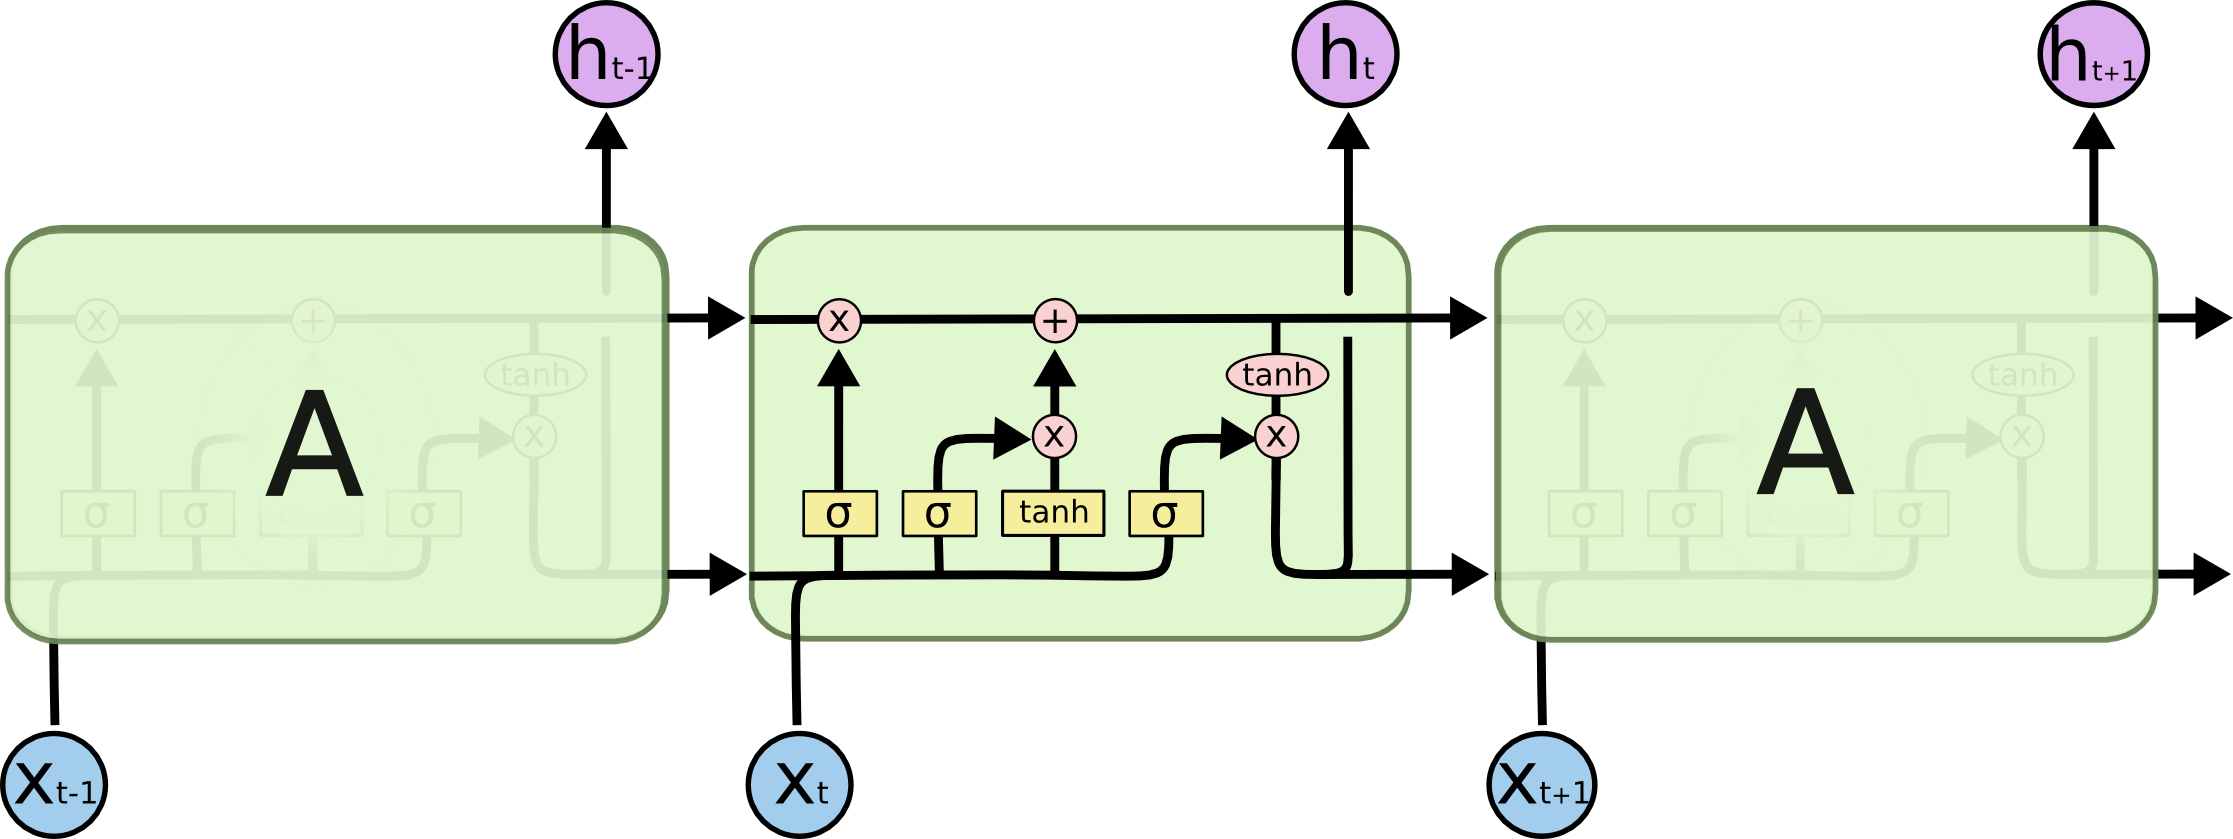
\includegraphics[width=\textwidth]{Figures/LSTM}}
\end{center}
\decoRule
\caption[LSTM architecture]{LSTM architecture.}
\label{fig:lstm}
\end{figure}

\section{Binary Classification}

The next sections describe the methodology applied to solve the binary classification problem using LSTMs

%-----------------------------------
%	SUBSECTION 1
%-----------------------------------
\subsection{Data Generation}

Before the ingestion of the data into the LSTM model, it has to be adapted to the architecture of the network.

Being \textit{samples} the total number of data, \textit{timesteps} the amount of rows to be ingested for each aircraft and \textit{features} the number of sensor data the input of the LSTM layer is defined by a tensor of shape:

\begin{verbatim}
    (samples, timesteps, features)
\end{verbatim}

The time steps used for the study will be 50, which means that for each aircraft batches of 50 time steps will be taken.
Using the \textit{zip} function over the data of the aircraft with id=1, which contains 192 cycles. The batches will be distributed this way:

\begin{verbatim}
    (0, 50)     -> from row 0 to row 50
    (1, 51)     -> from row 1 to row 51
    (2, 52)     -> from row 2 to row 52
    ...
    (111, 192)  -> from row 111 to row 192
\end{verbatim}

After the pre-processing, the input tensor will have the shape:

\begin{verbatim}
    (15631, 50, 25)
\end{verbatim}

To generate the labels, the values of the column \textit{label 1}, which was generated on the data preparation (see chapter \ref{Chapter3}), must be grouped by aircraft indicating if the engine failed within \textit{w1} cycles.

The result label tensor has the shape:

\begin{verbatim}
    (15631, 1)
\end{verbatim}

%-----------------------------------
%	SUBSECTION 2
%-----------------------------------

\subsection{Model definition}

As explained above, the architecture of the neural network is based on the use of LSTM layers. In this model two different LSTM layers are used to achieve better results.

To accomplish the binary classification, the output layer of the network is a Dense layer with a single output value. This value classifies between two different options: the aircraft will fail or not within the specified cycle.

To prevent over-fitting, two Dropout layers are concatenated after the output of both LSTM layers. This adds a regularization method that drops random units after the LSTM layers, avoiding the network to learn interdependent set of feature weights.

Finally, the loss function selected for this kind of classification problem is \textit{binary crossentropy} using \textit{Adam} as optimizer.

The diagram for the neural network is described in figure \ref{fig:binary-lstm-model}

\begin{figure}[H]
\centering
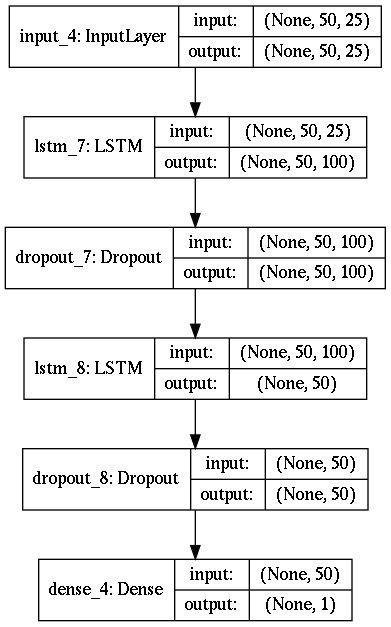
\includegraphics[scale=0.5]{Figures/binary-lstm-model}
\decoRule
\caption[Neural Network model for LSTM binary classification]{Neural Network model for LSTM binary classification.}
\label{fig:binary-lstm-model}
\end{figure}

\subsection{Training visualization}

Visualizing the output of the different layers of a network is one of the most useful tools to analyze the network performance. It could also help us to determine if the data analysis has been done correctly and allow us to see possible biases over the data distribution.

For the current network, the output of the last LSTM layer has been taken in account to do this analysis. The output of this layer is a tensor of size 50, which represents the hidden units of the LSTM. To extract the information contain by those celds, the \textit{Principal Component Analysis} (PCA) function has been chosen.

PCA is a mathematical function that allows us to summarize huge features sets. For this dissertation, two principal components has been configured. In figure \ref{fig:binary-lstm-pca} you can see a graphical representation of this components.

In this figure we can clearly see how the values conforms to main clusters of data. This has a lot of sense since we are trying to classify the data in two different groups.

\begin{figure}[H]
\centering
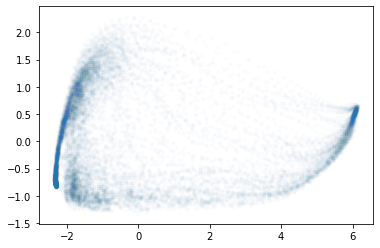
\includegraphics{Figures/lstm-visualization}
\decoRule
\caption[PCA applied over LSTM output]{PCA applied over LSTM output.}
\label{fig:binary-lstm-pca}
\end{figure}


\subsection{Results and model evaluation}

After the model is trained using batches of data of size 200. The validation split selected for the data is 5\%.

The evolution of the loss and accuracy during the model training can be seen in the figures \ref{fig:binary-lstm-loss} and \ref{fig:binary-lstm-acc}

The final accuracy obtained is 98\% so we can conclude that the network works very well for this task. To evaluate the results against the ground truth data a comparison graph has been generated. This graph can be seen in figure \ref{fig:binary-lstm-results}.

\begin{figure}[H]
\begin{center}
  \makebox[\textwidth]{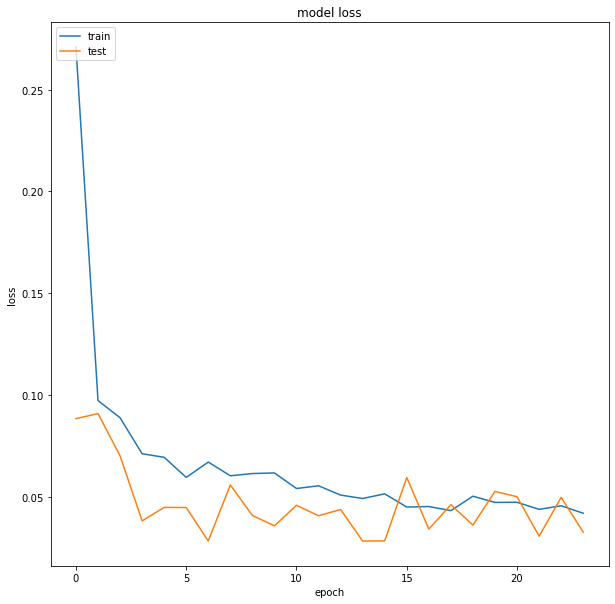
\includegraphics[width=\textwidth]{Figures/binary-lstm-loss}}
\end{center}
\decoRule
\caption[LSTM Binary Classification Model Loss]{LSTM Binary Classification Model Loss.}
\label{fig:binary-lstm-loss}\end{figure}

\begin{figure}[H]
\begin{center}
  \makebox[\textwidth]{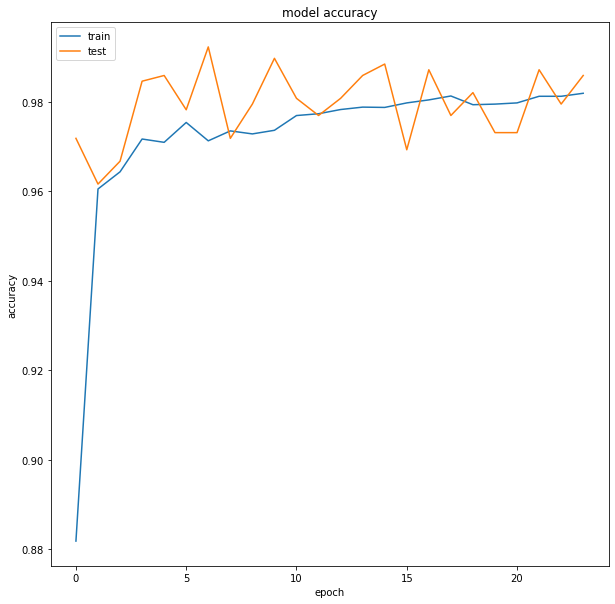
\includegraphics[width=\textwidth]{Figures/binary-lstm-acc}}
\end{center}
\decoRule
\caption[LSTM Binary Classification Model Accuracy]{LSTM Binary Classification Model Accuracy.}
\label{fig:binary-lstm-acc}
\end{figure}

\begin{figure}[H]
\begin{center}
  \makebox[\textwidth]{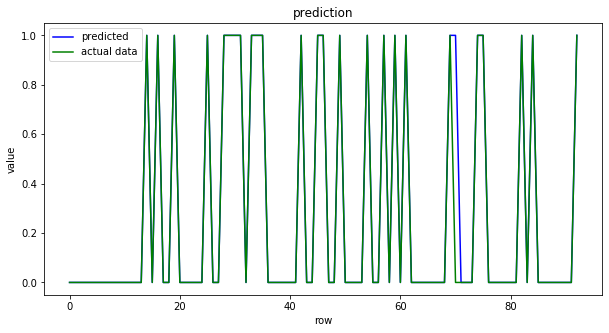
\includegraphics[width=\textwidth]{Figures/binary-lstm-results}}
\end{center}
\decoRule
\caption[Result comparison between Binary LSTM Model and Ground Truth data]{Result comparison between Binary LSTM Model and Ground Truth data.}
\label{fig:binary-lstm-results}
\end{figure}


\section{Regression Model}

The next sections describe the methodology applied to solve the regression problem using LSTMs


\subsection{Data Generation}

Before the ingestion of the data into the LSTM model, it has to be adapted to the architecture of the network.

Being \textit{samples} the total number of data, \textit{timesteps} the amount of rows to be ingested for each aircraft and \textit{features} the number of sensor data the input of the LSTM layer is defined by a tensor of shape:

\begin{verbatim}
    (samples, timesteps, features)
\end{verbatim}

The time steps used for the study will be 50, which means that for each aircraft batches of 50 time steps will be taken.
Using the \textit{zip} function over the data of the aircraft with id=1, which contains 192 cycles. The batches will be distributed this way:

\begin{verbatim}
    (0, 50)     -> from row 0 to row 50
    (1, 51)     -> from row 1 to row 51
    (2, 52)     -> from row 2 to row 52
    ...
    (111, 192)  -> from row 111 to row 192
\end{verbatim}

After the pre-processing, the input tensor will have the shape:

\begin{verbatim}
    (15631, 50, 25)
\end{verbatim}

For this type of regression model the labels are the values of the column \textit{RUL}, which was generated on the data preparation (see chapter \ref{Chapter3}).

The result label tensor has the shape:

\begin{verbatim}
    (15631, 1)
\end{verbatim}


\subsection{Model definition}

As explained above, the architecture of the neural network is based on the use of LSTM layers. In this model two different LSTM layers are used to achieve better results.

To accomplish the binary classification, the output layer of the network is a Dense layer with a single output value. This linear value is generated by the network output and represents the \textit{RUL} that the network calculates for an especific aircraft. Finally, an linear activation function is added to the last layer.

To prevent over-fitting, two Dropout layers are concatenated after the output of both LSTM layers. This adds a regularization method that drops random units after the LSTM layers, avoiding the network to learn interdependent set of feature weights.

The loss function selected for this kind of classification problem is \textit{binary crossentropy} using \textit{RMSProp} as optimizer.

For the regression model the metric used is \textit{MAE}, also, in this dissertation the \textit{Coefficient of Determination} (R squared) metric function has been implemented.

The diagram for the neural network is described in figure \ref{fig:regression-lstm-model}

\begin{figure}[H]
\centering
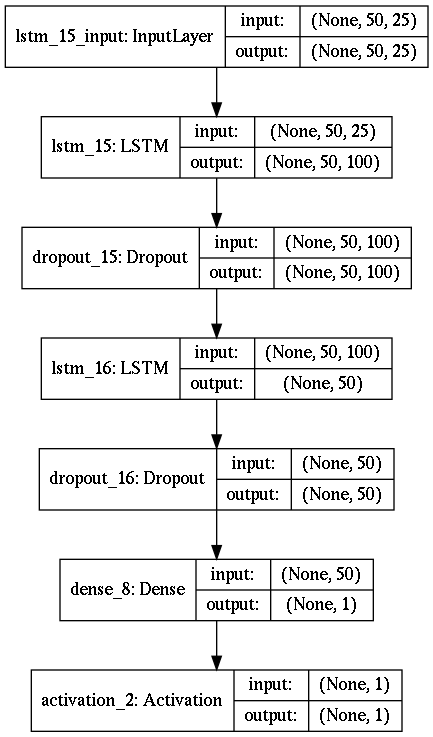
\includegraphics[scale=0.5]{Figures/regression-lstm-model}
\decoRule
\caption[LSTM Neural Network for regression model]{LSTM Neural Network for regression model.}
\label{fig:regression-lstm-model}
\end{figure}

\subsection{Results and model evaluation}

After the model is trained using batches of data of size 200. The validation split selected for the data is 5\%.

The evolution of the loss and metrics during the model training can be seen in the figures \ref{fig:regression-lstm-loss}, \ref{fig:regression-lstm-r2} and \ref{fig:regression-lstm-mae}

The final results obtained for \textit{MAE} and \textit{R-square} are 11.93 and 0.81 respectively.To evaluate the results against the ground truth data a comparison graph has been generated. This graph can be seen in figure \ref{fig:regression-lstm-results}.

\begin{figure}[H]
\begin{center}
  \makebox[\textwidth]{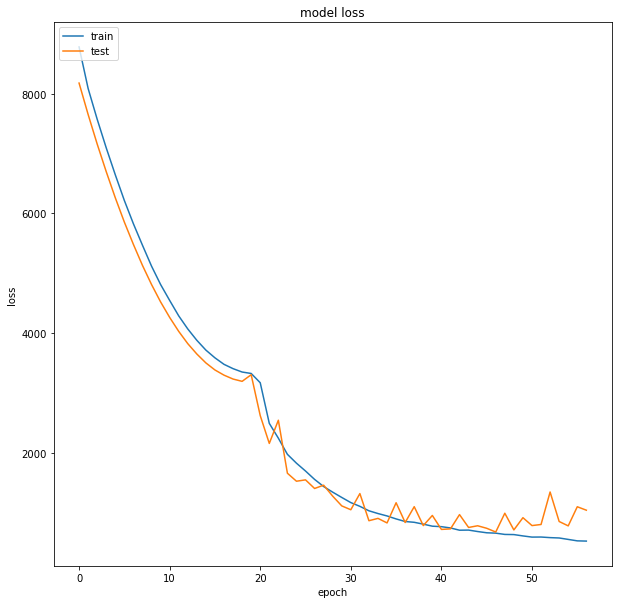
\includegraphics[width=\textwidth]{Figures/regression-lstm-loss}}
\end{center}
\decoRule
\caption[LSTM Regression Model Loss]{LSTM Regression Model Loss.}
\label{fig:regression-lstm-loss}\end{figure}

\begin{figure}[H]
\begin{center}
  \makebox[\textwidth]{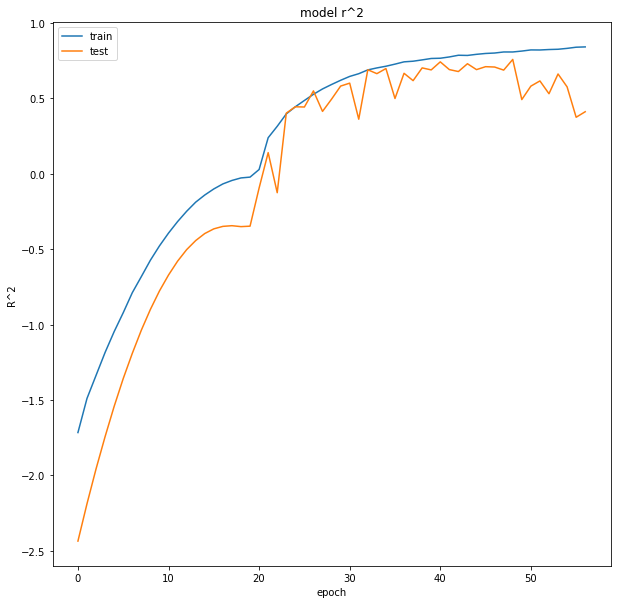
\includegraphics[width=\textwidth]{Figures/regression-lstm-r2}}
\end{center}
\decoRule
\caption[LSTM R2 model]{LSTM R2 model.}
\label{fig:regression-lstm-r2}
\end{figure}

\begin{figure}[H]
\begin{center}
  \makebox[\textwidth]{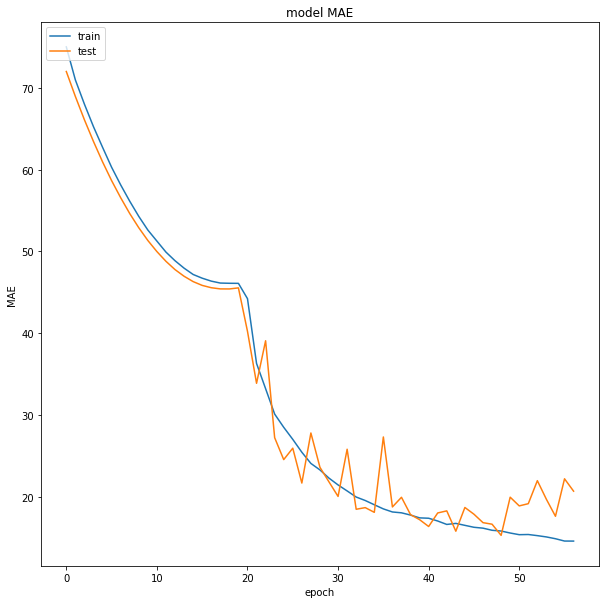
\includegraphics[width=\textwidth]{Figures/regression-lstm-mae}}
\end{center}
\decoRule
\caption[LSTM MAE model]{LSTM MAE model.}
\label{fig:regression-lstm-mae}
\end{figure}

\begin{figure}[H]
\begin{center}
  \makebox[\textwidth]{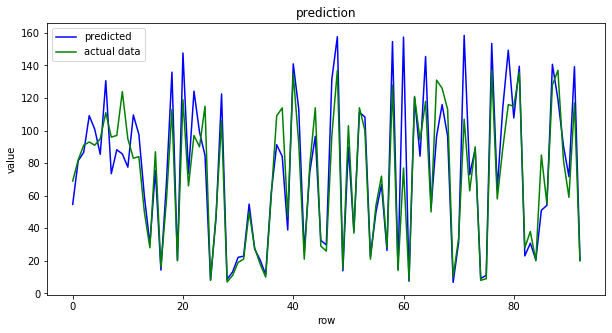
\includegraphics[width=\textwidth]{Figures/regression-lstm-results}}
\end{center}
\decoRule
\caption[Result comparison between Regression LSTM Model and Ground Truth data]{Result comparison between Regression LSTM Model and Ground Truth data.}
\label{fig:regression-lstm-results}
\end{figure}

%% Chapter Template

\chapter{Gated Recurrent Unit} % Main chapter title

\label{Chapter5} % Change X to a consecutive number; for referencing this chapter elsewhere, use \ref{ChapterX}

%----------------------------------------------------------------------------------------
%	SECTION 1
%----------------------------------------------------------------------------------------

\section{Understanding GRUs}

Gated recurrent units (GRUs) are a gating mechanism in recurrent neural networks, introduced in 2014 by Kyunghyun Cho et al \citation{Reference5}.

The GRU is like a LSTM with a forget gate but has fewer parameters than LSTM, as it lacks an output gate.

An scheme of a GRU architecture is described in figure \ref{fig:gru}.

\begin{figure}[H]
\begin{center}
  \makebox[\textwidth]{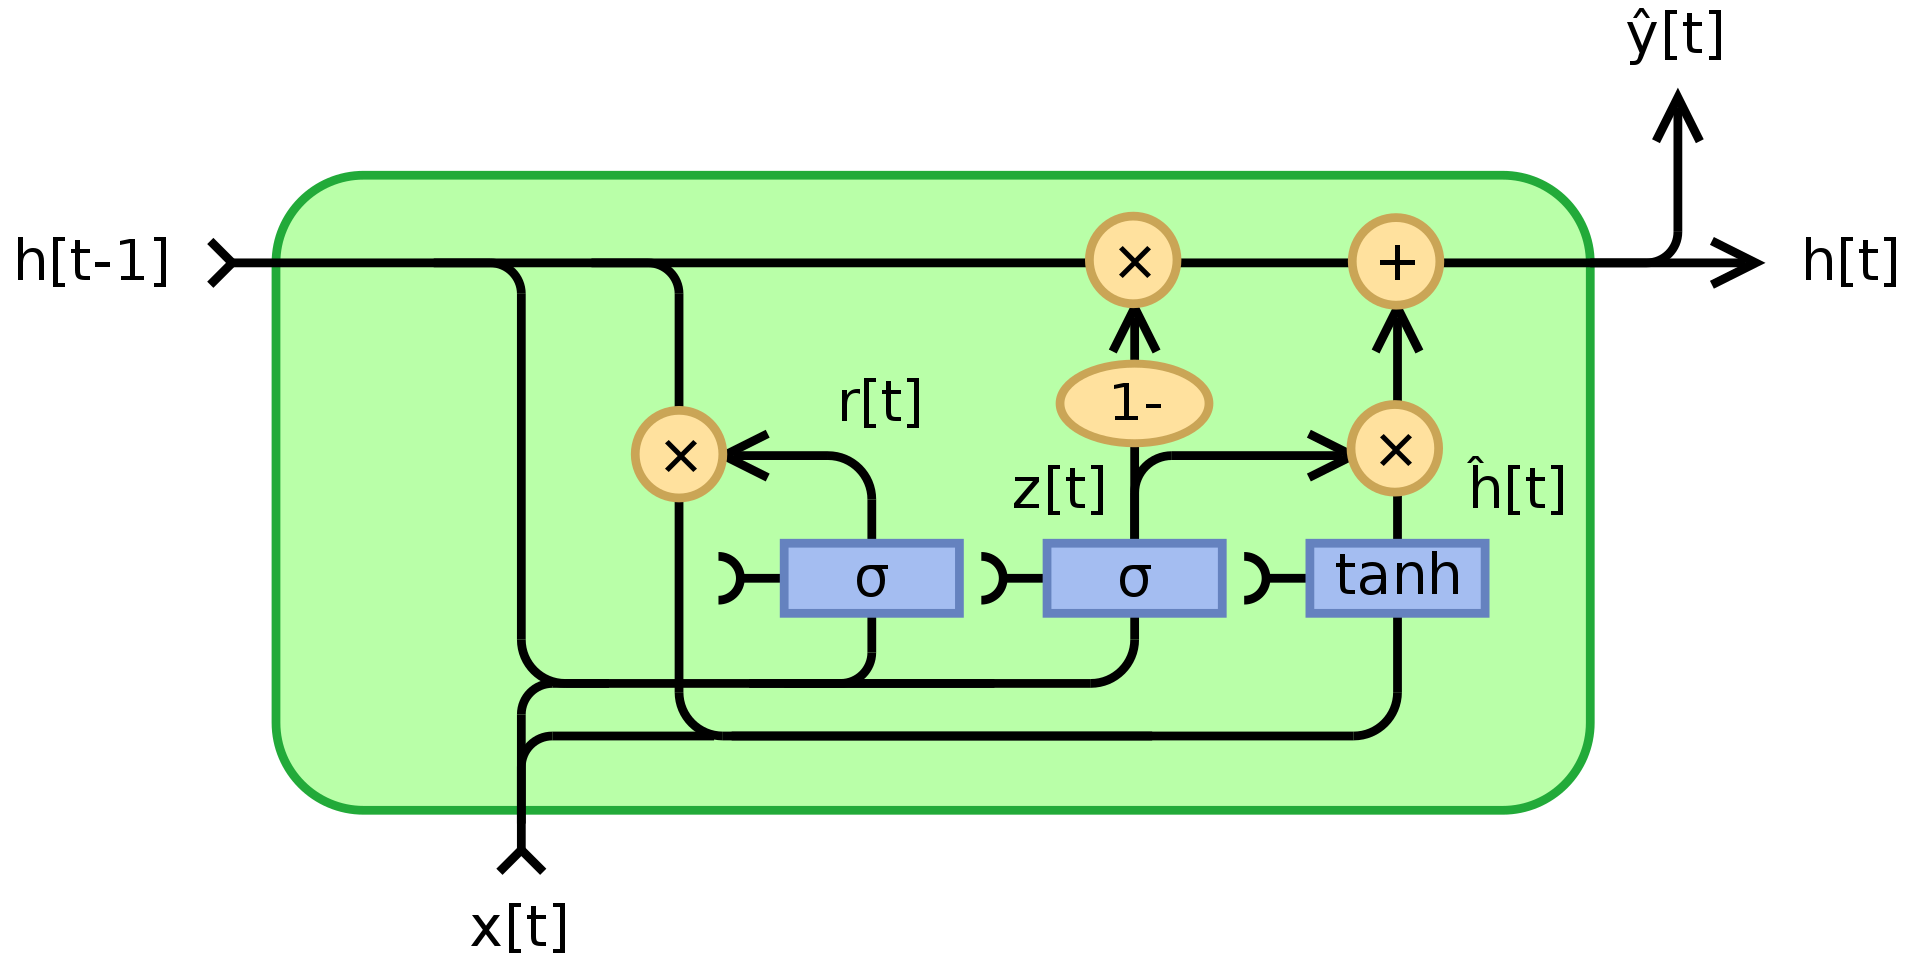
\includegraphics[width=\textwidth]{Figures/GRU}}
\end{center}
\decoRule
\caption[GRU architecture]{GRU architecture.}
\label{fig:gru}
\end{figure}

\section{Binary Classification}

The next sections describe the methodology applied to solve the binary classification problem using GRUs.

\subsection{Data Generation}

Before the ingestion of the data into the GRU model, it has to be adapted to the architecture of the network.

Being \textit{samples} the total number of data, \textit{timesteps} the amount of rows to be ingested for each aircraft and \textit{features} the number of sensor data the input of the GRU layer is defined by a tensor of shape:

\begin{verbatim}
    (samples, timesteps, features)
\end{verbatim}

The time steps used for the study will be 50, which means that for each aircraft batches of 50 time steps will be taken.
Using the \textit{zip} function over the data of the aircraft with id=1, which contains 192 cycles. The batches will be distributed this way:

\begin{verbatim}
    (0, 50)     -> from row 0 to row 50
    (1, 51)     -> from row 1 to row 51
    (2, 52)     -> from row 2 to row 52
    ...
    (111, 192)  -> from row 111 to row 192
\end{verbatim}

After the pre-processing, the input tensor will have the shape:

\begin{verbatim}
    (15631, 50, 25)
\end{verbatim}

To generate the labels, the values of the column \textit{label 1}, which was generated on the data preparation (see chapter \ref{Chapter3}), must be grouped by aircraft indicating if the engine failed within \textit{w1} cycles.

The result label tensor has the shape:

\begin{verbatim}
    (15631, 1)
\end{verbatim}

%-----------------------------------
%	SUBSECTION 2
%-----------------------------------

\subsection{Model definition}

This model is based on the previous one that focuses on the use of LSTM layers. This time the same architecture, loss and activation functions are used but all the LSTM layers are switched by GRU layers.

Instead of adding Dropout layers, the dropout field provided by the Keras API implementation of the GRU layers is used.

The diagram for the neural network is described in figure \ref{fig:binary-gru-model}

\begin{figure}[H]
\centering
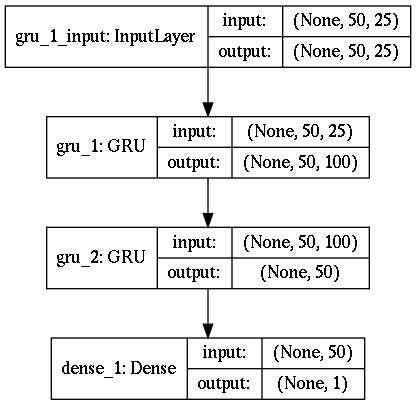
\includegraphics[scale=0.5]{Figures/binary-gru-model}
\decoRule
\caption[GRU Neural Network model for binary classification]{GRU Neural Network model for binary classification.}
\label{fig:binary-gru-model}
\end{figure}

\subsection{Training visualization}

As done in the previous model, the output of the second RNN layer has been visualized. In this case the second GRU layer is the one selected. The output of this layer is a tensor of size 50, which represents the hidden units of the GRU. To extract the information contain by those celds, the \textit{Principal Component Analysis} (PCA) function has been chosen.

In figure \ref{fig:binary-gru-pca} you can see a graphical representation of this components.

As happened with the LSTM model, two separated clusters can be seen in the image. This follows to the same conclusion, the data tends to split into two different options: the aircraft fails in a cycle or it doesn't.

\begin{figure}[H]
\centering
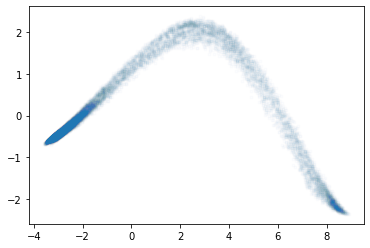
\includegraphics{Figures/gru-visualization}
\decoRule
\caption[PCA applied over GRU output]{PCA applied over GRU output.}
\label{fig:binary-gru-pca}
\end{figure}


\subsection{Results and model evaluation}

After the model is trained using batches of data of size 200. The validation split selected for the data is 5\%.

The evolution of the loss and accuracy during the model training can be seen in the figures \ref{fig:binary-gru-loss} and \ref{fig:binary-gru-acc}

The final accuracy obtained is 97\% so we can conclude that the network works very well for this task. To evaluate the results against the ground truth data a comparison graph has been generated. This graph can be seen in figure \ref{fig:binary-gru-results}.

\begin{figure}[H]
\begin{center}
  \makebox[\textwidth]{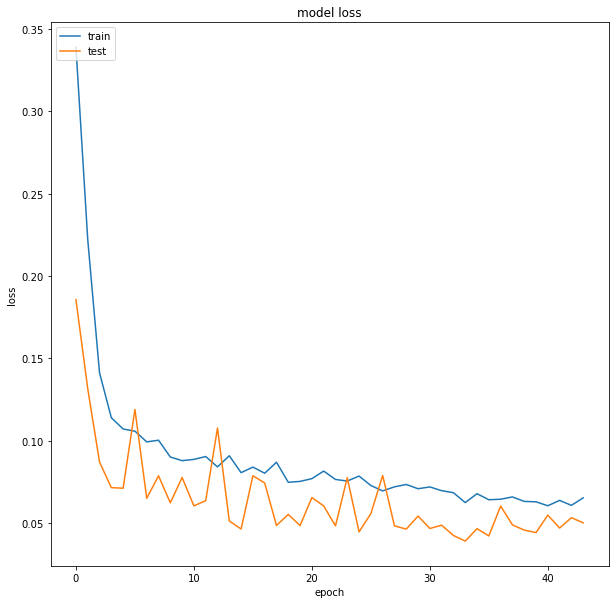
\includegraphics[width=\textwidth]{Figures/binary-gru-loss}}
\end{center}
\decoRule
\caption[GRU Binary Classification Model Loss]{GRU Binary Classification Model Loss.}
\label{fig:binary-gru-loss}\end{figure}

\begin{figure}[H]
\begin{center}
  \makebox[\textwidth]{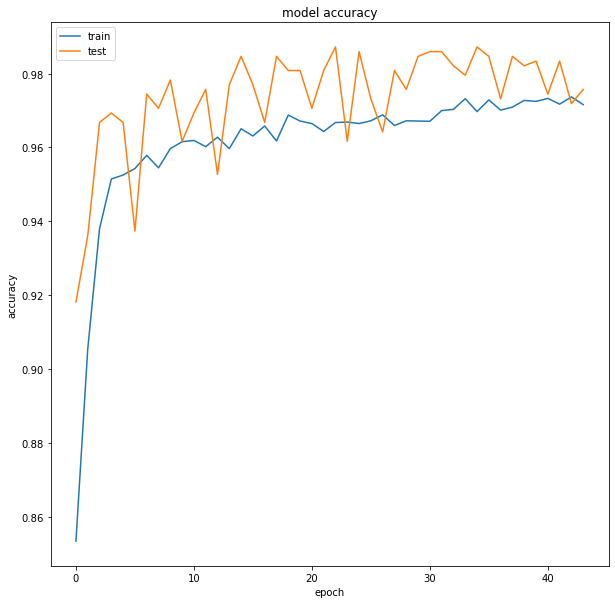
\includegraphics[width=\textwidth]{Figures/binary-gru-acc}}
\end{center}
\decoRule
\caption[GRU Binary Classification Model Accuracy]{GRU Binary Classification Model Accuracy.}
\label{fig:binary-gru-acc}
\end{figure}

\begin{figure}[H]
\begin{center}
  \makebox[\textwidth]{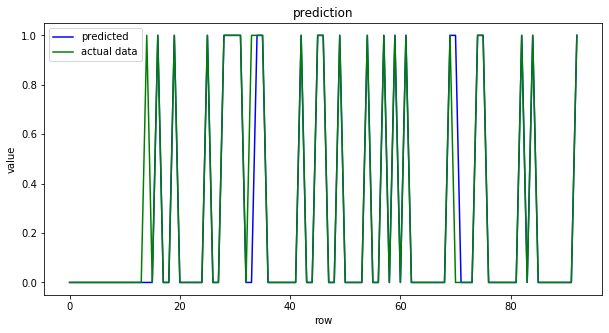
\includegraphics[width=\textwidth]{Figures/binary-gru-results}}
\end{center}
\decoRule
\caption[Result comparison between Binary GRU Model and Ground Truth data]{Result comparison between Binary GRU Model and Ground Truth data.}
\label{fig:binary-gru-results}
\end{figure}


\section{Regression Model}

The next sections describe the methodology applied to solve the regression problem using GRUs


\subsection{Data Generation}

Before the ingestion of the data into the GRU model, it has to be adapted to the architecture of the network.

Being \textit{samples} the total number of data, \textit{timesteps} the amount of rows to be ingested for each aircraft and \textit{features} the number of sensor data the input of the LSTM layer is defined by a tensor of shape:

\begin{verbatim}
    (samples, timesteps, features)
\end{verbatim}

The time steps used for the study will be 50, which means that for each aircraft batches of 50 time steps will be taken.
Using the \textit{zip} function over the data of the aircraft with id=1, which contains 192 cycles. The batches will be distributed this way:

\begin{verbatim}
    (0, 50)     -> from row 0 to row 50
    (1, 51)     -> from row 1 to row 51
    (2, 52)     -> from row 2 to row 52
    ...
    (111, 192)  -> from row 111 to row 192
\end{verbatim}

After the pre-processing, the input tensor will have the shape:

\begin{verbatim}
    (15631, 50, 25)
\end{verbatim}

For this type of regression model the labels are the values of the column \textit{RUL}, which was generated on the data preparation (see chapter \ref{Chapter3}).

The result label tensor has the shape:

\begin{verbatim}
    (15631, 1)
\end{verbatim}


\subsection{Model definition}

Like the binary one, this model has been created just replacing the LSTMs layers used in the previous chapter with GRU layers. The rest of the components of the model remain the same.

As a point, it is interesting to notice that in order to make the model converge, especific Dropout layers has been used instead that the features provided by the GRU layer API.

The diagram for the neural network is described in figure \ref{fig:regression-gru-model}

\begin{figure}[H]
\centering
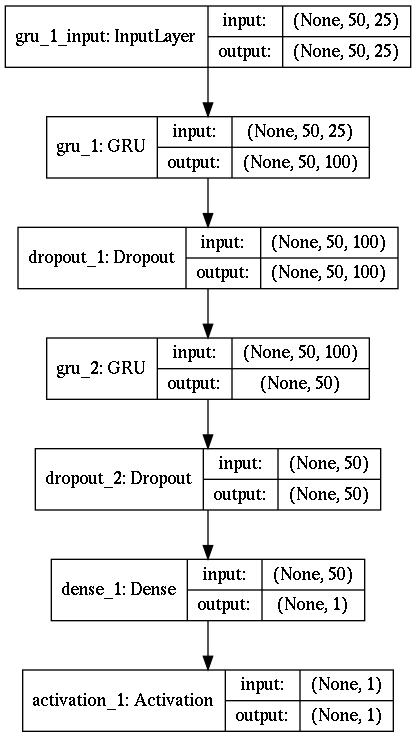
\includegraphics[scale=0.5]{Figures/regression-gru-model}
\decoRule
\caption[Neural Network for GRU regression model]{Neural Network for GRU regression model.}
\label{fig:regression-gru-model}
\end{figure}

\subsection{Results and model evaluation}

After the model is trained using batches of data of size 200. The validation split selected for the data is 5\%.

The evolution of the loss and metrics during the model training can be seen in the figures \ref{fig:regression-gru-loss}, \ref{fig:regression-gru-r2} and \ref{fig:regression-gru-mae}

The final results obtained for \textit{MAE} and \textit{R-square} are 13.70 and 0.81 respectively. To evaluate the results against the ground truth data a comparison graph has been generated. This graph can be seen in figure \ref{fig:regression-gru-results}.

\begin{figure}[H]
\begin{center}
  \makebox[\textwidth]{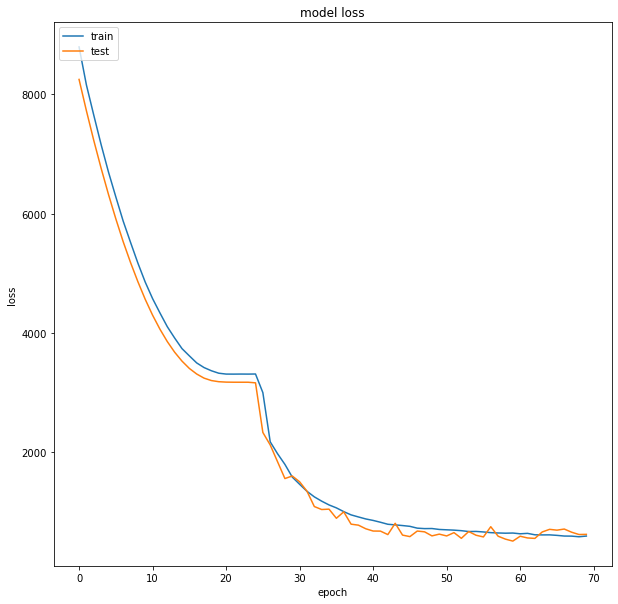
\includegraphics[width=\textwidth]{Figures/regression-gru-loss}}
\end{center}
\decoRule
\caption[GRU Regression Model Loss]{GRU Regression Model Loss.}
\label{fig:regression-gru-loss}\end{figure}

\begin{figure}[H]
\begin{center}
  \makebox[\textwidth]{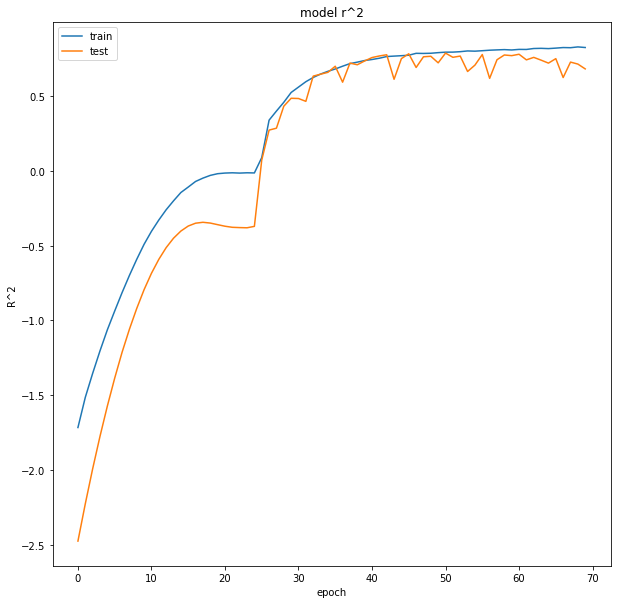
\includegraphics[width=\textwidth]{Figures/regression-gru-r2}}
\end{center}
\decoRule
\caption[GRU R2 model]{GRU R2 model.}
\label{fig:regression-gru-r2}
\end{figure}

\begin{figure}[H]
\begin{center}
  \makebox[\textwidth]{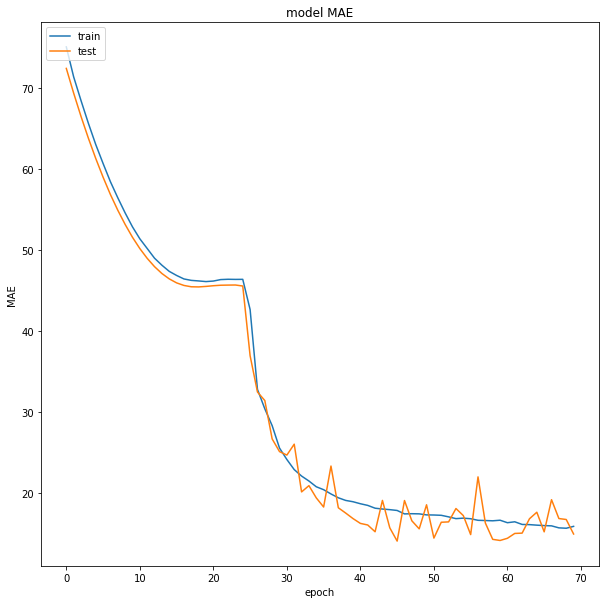
\includegraphics[width=\textwidth]{Figures/regression-gru-mae}}
\end{center}
\decoRule
\caption[GRU MAE model]{GRU MAE model.}
\label{fig:regression-gru-mae}
\end{figure}

\begin{figure}[H]
\begin{center}
  \makebox[\textwidth]{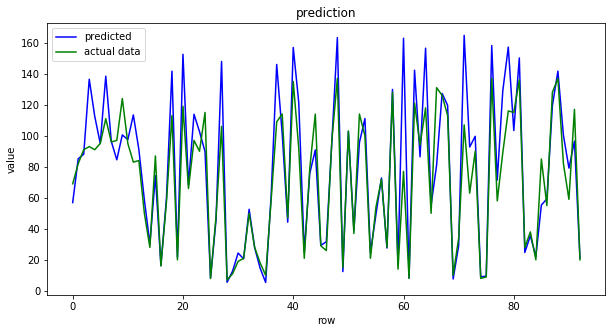
\includegraphics[width=\textwidth]{Figures/regression-gru-results}}
\end{center}
\decoRule
\caption[Result comparison between Regression GRU Model and Ground Truth data]{Result comparison between Regression GRU Model and Ground Truth data.}
\label{fig:regression-gru-results}
\end{figure}


%----------------------------------------------------------------------------------------
%	THESIS CONTENT - APPENDICES
%----------------------------------------------------------------------------------------

\appendix % Cue to tell LaTeX that the following "chapters" are Appendices

% Include the Appendices of the thesis as separate files from the Appendices folder
% Uncomment the lines as you write the Appendices

% Appendix A

\chapter{Code And Templates} % Main appendix title

\label{AppendixA} % For referencing this appendix elsewhere, use \ref{AppendixA}

\section{Source code}

All the code used for the implementation of this dissertation can be found on this GitHub \href{https://github.com/hperezblasco/mbit-tfm}{repository}.

\section{Template}

This dissertation was written using \textit{LaTex} based on the Master/Doctoral Thesis template made by Steve R. Gunn and Sunil Patel. The template can be found \href{https://www.latextemplates.com/template/masters-doctoral-thesis}{here}.

%\input{Appendices/AppendixB}
%\input{Appendices/AppendixC}

%----------------------------------------------------------------------------------------
%	BIBLIOGRAPHY
%----------------------------------------------------------------------------------------

\printbibliography[heading=bibintoc]

%----------------------------------------------------------------------------------------

\end{document}  
